\newpage

\begin{figure}[h]
    \centering
    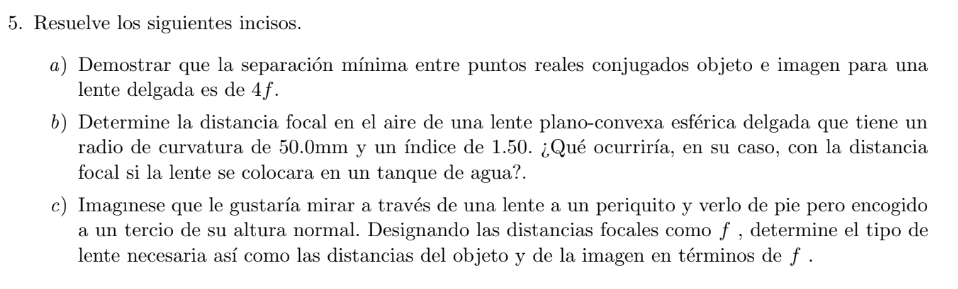
\includegraphics[width=1\linewidth]{5en.png}
\end{figure}

Sabemos que la ecuación de las lentes delgadas es:

\[
\frac{1}{s} + \frac{1}{s_i} = \frac{1}{f}.
\]

La distancia entre el objeto y la imagen está dada por:

\[
d = s + s_i.
\]

Para encontrar la separación mínima, expresamos \( s_i \) en términos de \( s \):

\[
s_i = \frac{sf}{s - f}.
\]

Sustituyéndolo en \( d \):

\[
d = s + \frac{sf}{s - f}.
\]

Para minimizar \( d \), derivamos con respecto a \( s \) y buscamos el mínimo:

\[
\frac{d}{ds} \left( s + \frac{sf}{s - f} \right) = 1 + \frac{f(s - f) - sf}{(s - f)^2} = 1 + \frac{-f^2}{(s - f)^2}.
\]

Igualamos a cero:

\[
1 - \frac{f^2}{(s - f)^2} = 0.
\]

\[
(s - f)^2 = f^2 \Rightarrow s - f = \pm f.
\]

Tomamos el valor positivo porque buscamos una distancia real:

\[
s = 2f.
\]

Sustituyendo en la ecuación de la imagen:

\[
s_i = \frac{(2f) f}{2f - f} = \frac{2f^2}{f} = 2f.
\]

Por lo tanto:

\[
d = s + s_i = 2f + 2f = 4f.
\]

QED \\

La distancia focal de una lente delgada está dada por la ecuación del fabricante de lentes:

\[
\frac{1}{f} = (n - 1) \left( \frac{1}{R_1} - \frac{1}{R_2} \right).
\]

Dado que la lente es plano-convexa, tenemos:

- \( R_1 = 50.0 \) mm \( = 5.00 \) cm,\\
- \( R_2 = \infty \) (superficie plana),\\
- Índice de refracción de la lente: \( n = 1.50 \).\\

Sustituyo:

\[
\frac{1}{f} = (1.50 - 1) \left( \frac{1}{5.00} - \frac{1}{\infty} \right).
\]

\[
\frac{1}{f} = 0.50 \times \frac{1}{5.00} = \frac{0.50}{5.00} = 0.10.
\]

\[
f = 10.0 \text{ cm}.
\]

Si la lente se coloca en agua, su nuevo índice de refracción relativo será:

\[
n' = \frac{n_{\text{lente}}}{n_{\text{agua}}} = \frac{1.50}{1.33} \approx 1.13.
\]

Usamos la ecuación del fabricante de lentes nuevamente:

\[
\frac{1}{f'} = (1.13 - 1) \left( \frac{1}{5.00} - \frac{1}{\infty} \right).
\]

\[
\frac{1}{f'} = 0.13 \times \frac{1}{5.00} = \frac{0.13}{5.00} = 0.026.
\]

\[
f' \approx 38.5 \text{ cm}.
\]

Si la imagen es un tercio del tamaño del objeto:

\[
M = \frac{-s_i}{s} = \frac{1}{3}.
\]

De aquí:

\[
s_i = -\frac{s}{3}.
\]

Sustituyendo en la ecuación de las lentes:

\[
\frac{1}{s} + \frac{1}{-\frac{s}{3}} = \frac{1}{f}.
\]

Calculamos el denominador:

\[
\frac{1}{s} - \frac{3}{s} = \frac{1}{f}.
\]

\[
\frac{-2}{s} = \frac{1}{f}.
\]

\[
s = -2f.
\]

Sustituyendo en \( s_i = -\frac{s}{3} \):

\[
s_i = -\frac{-2f}{3} = \frac{2f}{3}.
\]

De aquí se sigue que \\
- \( s \) es negativo: el objeto está del mismo lado que la imagen.   \\
- \( s_i \) es positivo: la imagen está del otro lado de la lente.  \\
- La imagen es más pequeña y derecha. \\

Esto sugiere que la lente es divergente (cóncava), ya que este tipo de lentes siempre produce imágenes virtuales, derechas y más pequeñas.